\documentclass{standalone}
\usepackage{tikz}
\usetikzlibrary{patterns, positioning}


\begin{document}
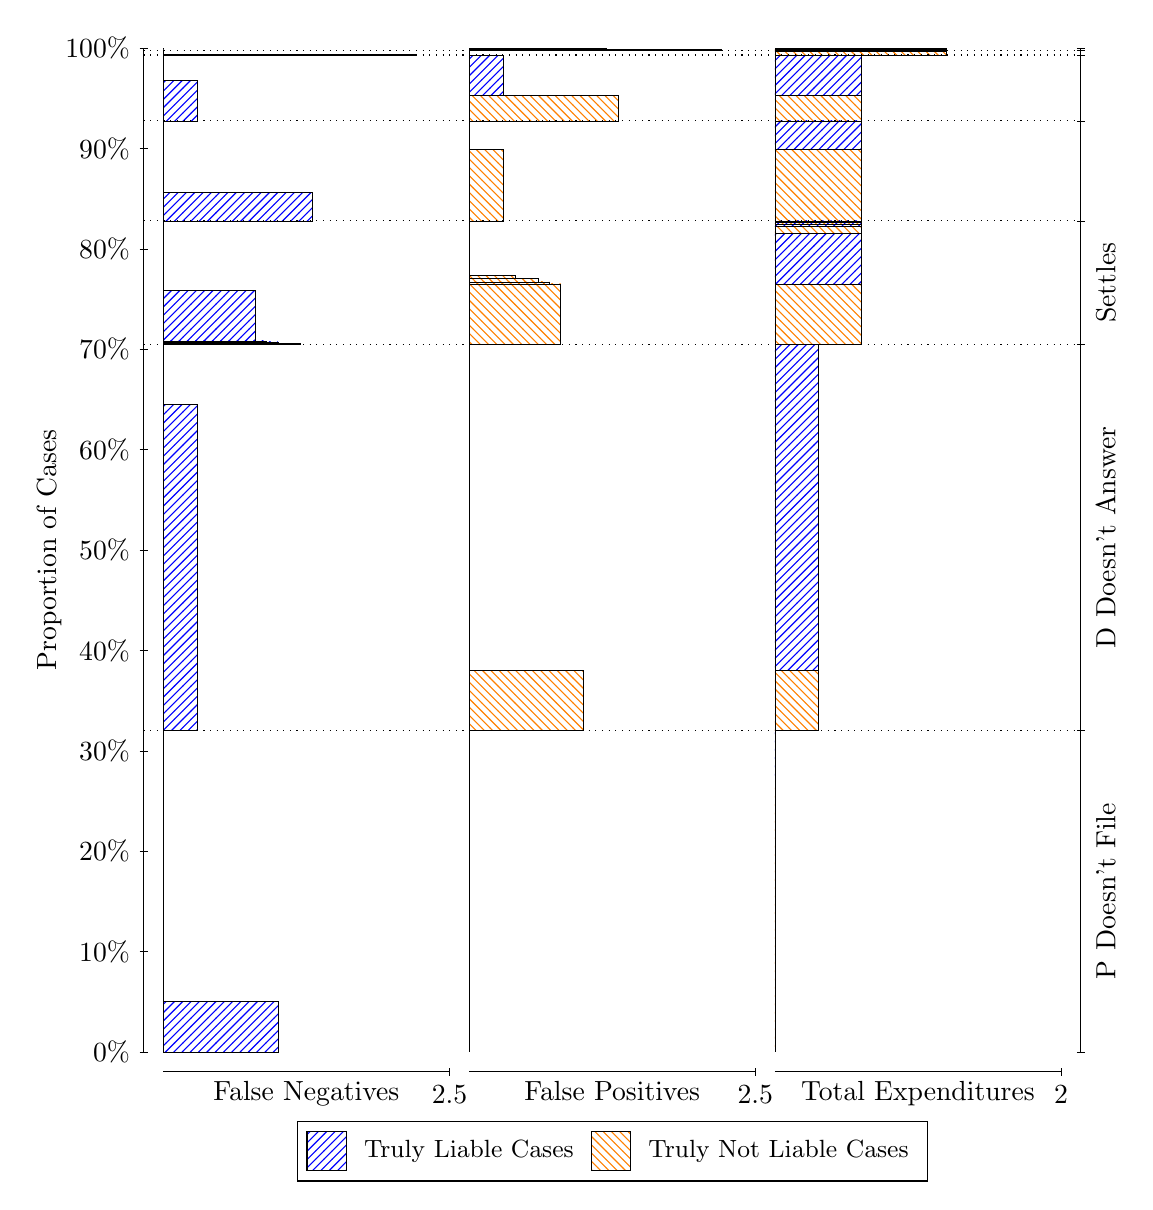
\begin{tikzpicture}
\draw[black, very thin] (1.5,1.75) -- (1.5,14.5);
\node[rotate=90, text=black, anchor=center] at (0.3, 8.125) {Proportion of Cases};
\draw[black, very thin] (1.45,1.75) -- (1.55,1.75);
\node[text=black, anchor=east] at (1.45, 1.75) {0\%};
\draw[black, very thin] (1.45,3.025) -- (1.55,3.025);
\node[text=black, anchor=east] at (1.45, 3.025) {10\%};
\draw[black, very thin] (1.45,4.3) -- (1.55,4.3);
\node[text=black, anchor=east] at (1.45, 4.3) {20\%};
\draw[black, very thin] (1.45,5.575) -- (1.55,5.575);
\node[text=black, anchor=east] at (1.45, 5.575) {30\%};
\draw[black, very thin] (1.45,6.85) -- (1.55,6.85);
\node[text=black, anchor=east] at (1.45, 6.85) {40\%};
\draw[black, very thin] (1.45,8.125) -- (1.55,8.125);
\node[text=black, anchor=east] at (1.45, 8.125) {50\%};
\draw[black, very thin] (1.45,9.4) -- (1.55,9.4);
\node[text=black, anchor=east] at (1.45, 9.4) {60\%};
\draw[black, very thin] (1.45,10.675) -- (1.55,10.675);
\node[text=black, anchor=east] at (1.45, 10.675) {70\%};
\draw[black, very thin] (1.45,11.95) -- (1.55,11.95);
\node[text=black, anchor=east] at (1.45, 11.95) {80\%};
\draw[black, very thin] (1.45,13.225) -- (1.55,13.225);
\node[text=black, anchor=east] at (1.45, 13.225) {90\%};
\draw[black, very thin] (1.45,14.5) -- (1.55,14.5);
\node[text=black, anchor=east] at (1.45, 14.5) {100\%};

\draw[black, very thin] (13.4,1.75) -- (13.4,14.5);
\draw[black, very thin] (13.35,1.75) -- (13.45,1.75);
\node[anchor=west] at (13.35, 1.75) {};
\draw[black, very thin] (13.35,5.8364) -- (13.45,5.8364);
\node[anchor=west] at (13.35, 5.8364) {};
\draw[black, very thin] (13.35,10.735) -- (13.45,10.735);
\node[anchor=west] at (13.35, 10.735) {};
\draw[black, very thin] (13.35,12.305) -- (13.45,12.305);
\node[anchor=west] at (13.35, 12.305) {};
\draw[black, very thin] (13.35,13.575) -- (13.45,13.575);
\node[anchor=west] at (13.35, 13.575) {};
\draw[black, very thin] (13.35,14.411) -- (13.45,14.411);
\node[anchor=west] at (13.35, 14.411) {};
\draw[black, very thin] (13.35,14.472) -- (13.45,14.472);
\node[anchor=west] at (13.35, 14.472) {};
\draw[black, very thin] (13.35,14.5) -- (13.45,14.5);
\node[anchor=west] at (13.35, 14.5) {};

\draw[black, very thin, pattern color=blue, pattern=north east lines] (1.75,1.75) rectangle (3.2033,2.3951);
\draw[black, very thin, pattern color=orange, pattern=north west lines] (1.75,2.3951) rectangle (1.75,5.8364);
\draw[black, very thin, pattern color=blue, pattern=north east lines] (1.75,5.8364) rectangle (2.186,9.9744);
\draw[black, very thin, pattern color=orange, pattern=north west lines] (1.75,9.9744) rectangle (1.75,10.735);
\draw[black, very thin, pattern color=blue, pattern=north east lines] (1.75,10.735) rectangle (3.494,10.746);
\draw[black, very thin, pattern color=blue, pattern=north east lines] (1.75,10.746) rectangle (3.3487,10.748);
\draw[black, very thin, pattern color=blue, pattern=north east lines] (1.75,10.748) rectangle (3.2033,10.769);
\draw[black, very thin, pattern color=blue, pattern=north east lines] (1.75,10.769) rectangle (3.058,10.782);
\draw[black, very thin, pattern color=blue, pattern=north east lines] (1.75,10.782) rectangle (2.9127,11.426);
\draw[black, very thin, pattern color=orange, pattern=north west lines] (1.75,11.426) rectangle (1.75,12.305);
\draw[black, very thin, pattern color=blue, pattern=north east lines] (1.75,12.305) rectangle (3.6393,12.663);
\draw[black, very thin, pattern color=orange, pattern=north west lines] (1.75,12.663) rectangle (1.75,13.575);
\draw[black, very thin, pattern color=blue, pattern=north east lines] (1.75,13.575) rectangle (2.186,14.089);
\draw[black, very thin, pattern color=orange, pattern=north west lines] (1.75,14.089) rectangle (1.75,14.411);
\draw[black, very thin, pattern color=blue, pattern=north east lines] (1.75,14.411) rectangle (4.9473,14.423);
\draw[black, very thin, pattern color=orange, pattern=north west lines] (1.75,14.423) rectangle (1.75,14.472);
\draw[black, very thin, pattern color=orange, pattern=north west lines] (1.75,14.472) rectangle (1.75,14.483);
\draw[black, very thin, pattern color=blue, pattern=north east lines] (1.75,14.483) rectangle (1.75,14.5);
\draw[black, very thin, pattern color=orange, pattern=north west lines] (5.6333,1.75) rectangle (5.6333,5.1913);
\draw[black, very thin, pattern color=blue, pattern=north east lines] (5.6333,5.1913) rectangle (5.6333,5.8364);
\draw[black, very thin, pattern color=orange, pattern=north west lines] (5.6333,5.8364) rectangle (7.0867,6.5975);
\draw[black, very thin, pattern color=blue, pattern=north east lines] (5.6333,6.5975) rectangle (5.6333,10.735);
\draw[black, very thin, pattern color=orange, pattern=north west lines] (5.6333,10.735) rectangle (6.796,11.505);
\draw[black, very thin, pattern color=orange, pattern=north west lines] (5.6333,11.505) rectangle (6.6507,11.529);
\draw[black, very thin, pattern color=orange, pattern=north west lines] (5.6333,11.529) rectangle (6.5053,11.57);
\draw[black, very thin, pattern color=orange, pattern=north west lines] (5.6333,11.57) rectangle (6.36,11.577);
\draw[black, very thin, pattern color=orange, pattern=north west lines] (5.6333,11.577) rectangle (6.2147,11.614);
\draw[black, very thin, pattern color=blue, pattern=north east lines] (5.6333,11.614) rectangle (5.6333,12.305);
\draw[black, very thin, pattern color=orange, pattern=north west lines] (5.6333,12.305) rectangle (6.0693,13.216);
\draw[black, very thin, pattern color=blue, pattern=north east lines] (5.6333,13.216) rectangle (5.6333,13.575);
\draw[black, very thin, pattern color=orange, pattern=north west lines] (5.6333,13.575) rectangle (7.5227,13.897);
\draw[black, very thin, pattern color=blue, pattern=north east lines] (5.6333,13.897) rectangle (6.0693,14.411);
\draw[black, very thin, pattern color=orange, pattern=north west lines] (5.6333,14.411) rectangle (5.6333,14.46);
\draw[black, very thin, pattern color=blue, pattern=north east lines] (5.6333,14.46) rectangle (5.6333,14.472);
\draw[black, very thin, pattern color=orange, pattern=north west lines] (5.6333,14.472) rectangle (8.8307,14.483);
\draw[black, very thin, pattern color=blue, pattern=north east lines] (5.6333,14.483) rectangle (7.3773,14.5);
\draw[black, very thin, pattern color=orange, pattern=north west lines] (9.5167,1.75) rectangle (9.5167,5.1913);
\draw[black, very thin, pattern color=blue, pattern=north east lines] (9.5167,5.1913) rectangle (9.5167,5.8364);
\draw[black, very thin, pattern color=orange, pattern=north west lines] (9.5167,5.8364) rectangle (10.062,6.5975);
\draw[black, very thin, pattern color=blue, pattern=north east lines] (9.5167,6.5975) rectangle (10.062,10.735);
\draw[black, very thin, pattern color=orange, pattern=north west lines] (9.5167,10.735) rectangle (10.607,11.505);
\draw[black, very thin, pattern color=blue, pattern=north east lines] (9.5167,11.505) rectangle (10.607,12.148);
\draw[black, very thin, pattern color=orange, pattern=north west lines] (9.5167,12.148) rectangle (10.607,12.234);
\draw[black, very thin, pattern color=blue, pattern=north east lines] (9.5167,12.234) rectangle (10.607,12.268);
\draw[black, very thin, pattern color=orange, pattern=north west lines] (9.5167,12.268) rectangle (10.607,12.292);
\draw[black, very thin, pattern color=blue, pattern=north east lines] (9.5167,12.292) rectangle (10.607,12.305);
\draw[black, very thin, pattern color=orange, pattern=north west lines] (9.5167,12.305) rectangle (10.607,13.216);
\draw[black, very thin, pattern color=blue, pattern=north east lines] (9.5167,13.216) rectangle (10.607,13.575);
\draw[black, very thin, pattern color=orange, pattern=north west lines] (9.5167,13.575) rectangle (10.607,13.897);
\draw[black, very thin, pattern color=blue, pattern=north east lines] (9.5167,13.897) rectangle (10.607,14.411);
\draw[black, very thin, pattern color=orange, pattern=north west lines] (9.5167,14.411) rectangle (11.697,14.46);
\draw[black, very thin, pattern color=blue, pattern=north east lines] (9.5167,14.46) rectangle (11.697,14.472);
\draw[black, very thin, pattern color=orange, pattern=north west lines] (9.5167,14.472) rectangle (11.697,14.483);
\draw[black, very thin, pattern color=blue, pattern=north east lines] (9.5167,14.483) rectangle (11.697,14.5);
\draw[black, dotted] (1.5,5.8364) -- (13.4,5.8364);
\draw[black, dotted] (1.5,10.735) -- (13.4,10.735);
\draw[black, dotted] (1.5,12.305) -- (13.4,12.305);
\draw[black, dotted] (1.5,13.575) -- (13.4,13.575);
\draw[black, dotted] (1.5,14.411) -- (13.4,14.411);
\draw[black, dotted] (1.5,14.472) -- (13.4,14.472);
\draw[black, very thin] (1.75,1.5) -- (5.3833,1.5);
\node[text=black, anchor=north] at (3.5667, 1.5) {False Negatives};
\draw[black, very thin] (5.3833,1.45) -- (5.3833,1.55);
\node[text=black, anchor=north] at (5.3833, 1.45) {2.5};

\draw[black, very thin] (5.6333,1.5) -- (9.2667,1.5);
\node[text=black, anchor=north] at (7.45, 1.5) {False Positives};
\draw[black, very thin] (9.2667,1.45) -- (9.2667,1.55);
\node[text=black, anchor=north] at (9.2667, 1.45) {2.5};

\draw[black, very thin] (9.5167,1.5) -- (13.15,1.5);
\node[text=black, anchor=north] at (11.333, 1.5) {Total Expenditures};
\draw[black, very thin] (13.15,1.45) -- (13.15,1.55);
\node[text=black, anchor=north] at (13.15, 1.45) {2};

\node[text=black, centered, rotate=90] at (13.72, 3.7932) {P Doesn't File};
\node[text=black, centered, rotate=90] at (13.72, 8.2859) {D Doesn't Answer};
\node[text=black, centered, rotate=90] at (13.72, 11.52) {Settles};





\draw (7.449999999999999,1.5) node[draw=none] (baseCoordinate) {};
\begin{scope}[align=center]
        \matrix[scale=0.5, draw=black, below=0.5cm of baseCoordinate, nodes={draw}, column sep=0.1cm]{
            \node[rectangle, draw, minimum width=0.5cm, minimum height=0.5cm, pattern color=blue, pattern=north east lines] {}; &
            \node[draw=none, font=\small, text=black] (B) {Truly Liable Cases}; &
            \node[rectangle, draw, minimum width=0.5cm, minimum height=0.5cm, pattern color=orange, pattern=north west lines] {}; &
            \node[draw=none, font=\small, text=black] (B) {Truly Not Liable Cases}; \\
            };
\end{scope}

\end{tikzpicture}
\end{document}